\section{\sys{} Overview}
\label{sec:overv}

%This section shall look into the principle of each component in Processing Runtime subsystem, putting forth a full-fledged system.

\subsection{Problem Formulation}
% {user, blog, user-blog} => model
% query (a user u, a blog b that is created or forwarded by u's friend)
% returns: Y/N u shall forward b 

We consider people's \retg{} behavior in social media.
For simplicity, with a given user, we assume that blogs created or \retd{} by his/her followees cover the overall candidates, from which the said user may \ret{}.
All our results could straightforwardly generalize to alternative candidate scopes.
%e.g., the like/unlike behavior against the candidate of remarking [double check the network language; register a Facebook]
%e.g., positive comments in the overall comments

\begin{definition}
\label{def:blog}
A blog $B = (O, T, M, R)$ consists of the owner $O$ (a.k.a. user in this paper) to whom $B$ belongs (either created or \retd{}), the timestamp $T$ showing when $B$ is generated, the blog message $M$ and a bit $R$ denoting $B$ is \retd{} (1) or originally created (0) by the owner $O$.
\end{definition}

\begin{comment}
\begin{definition}
A blog $B = (O, T, M, C)$ consists of the owner $O$ to whom $B$ belongs (either created or \retd{}), the timestamp $T$ showing when $B$ is generated, the blog message $M$ and a set of counters $C_s(B) = \{\#comment,\ \#like,\ \#\ret{}\}$ regarding the number of being commented, liked, and \retd{}.
\end{definition}
\end{comment}

\begin{definition}
\label{def:user}
A user $U = (B_s, R_s, E_s)$ consists of three sets regarding the user's blogs $B_s$, followers $R_s$ and followees $E_s$ separately.
Each follower/followee per se refers to a user.
\end{definition}

The mapping between blog $B$ and user $U$ is a bilateral operation, i.e., $U = O(B)$ and $B \in B_s(U)$, through ID(s) of user and blog respectively.

Informally, providing a set of users $\{U\}$ and the associated blogs $\{B\}$, as well as a blog query $b$ and a follower of $O(b)$ written as $f$, i.e., $f \in R_s(O(b))$, \sys{} shall build a \retg{} model for $(\{U\},\ \{B\})$, upon which Y/N is returned regarding whether $f$ shall \ret{} $b$.


\subsection{\sys{} Framework}
\sys{} is designed from the ground up as a system for modeling users' \retg{} behavior in social media.
Figure \ref{fig:framework} shows the architectural components of \sys{}, comprising three subsystems: Data Storage, Processing Runtime and Profile Demonstrator.
 
\begin{figure}[!htb]
\centering
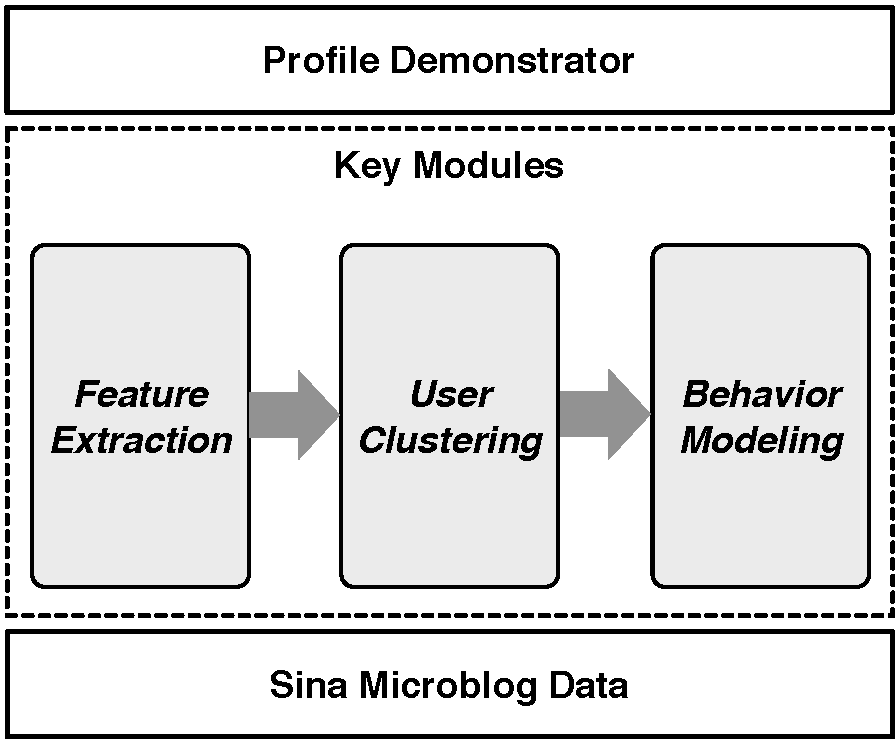
\includegraphics[width=.96\linewidth]{figures/architecture}
\caption{\sys{} Architecture}
\label{fig:framework}
\end{figure}


% #like and #comment are saved; could generalize \sys{} to model the liking behavior (among commented blogs)
\begin{comment}
\begin{figure}[!htb]
\centering
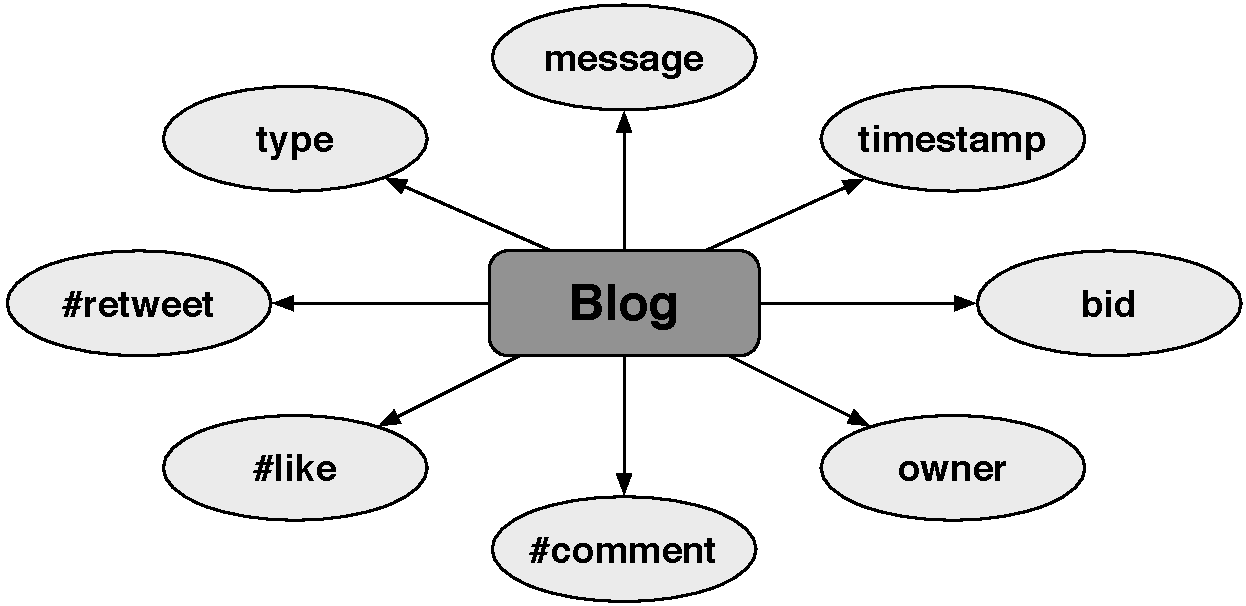
\includegraphics[width=.99\linewidth]{figures/microblog}
\caption{Blog Data in \sys{}}
\label{fig:blog}
\end{figure}
\end{comment}

\begin{comment}
\begin{figure}[!htb]
\centering
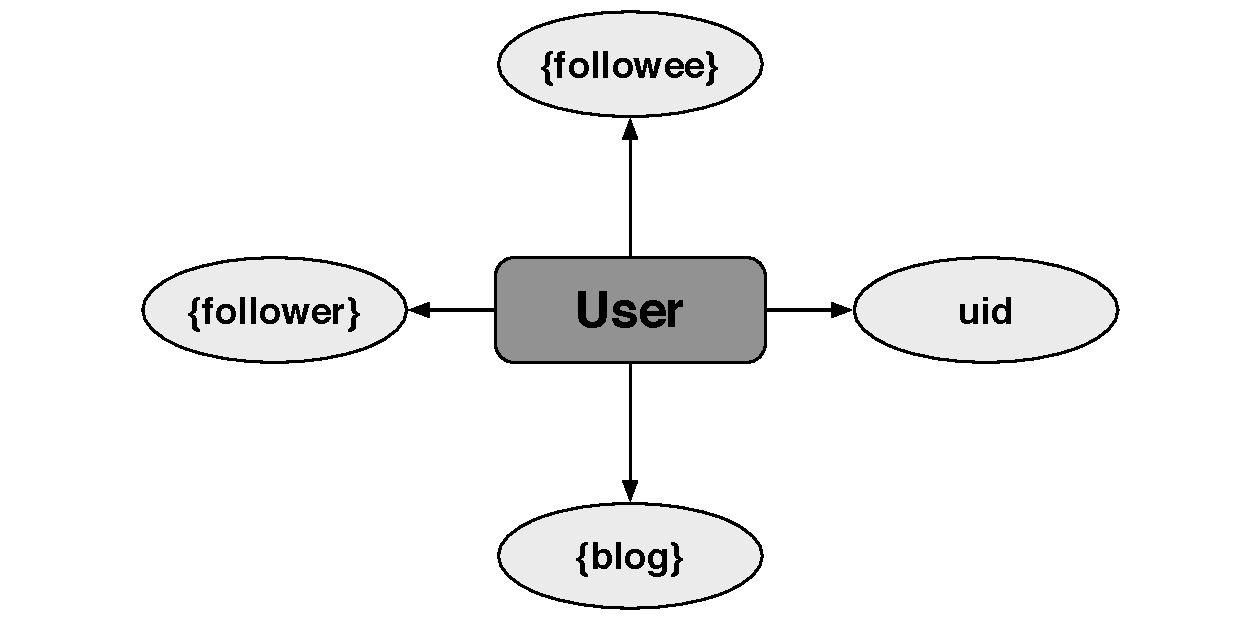
\includegraphics[width=.99\linewidth]{figures/user}
\caption{User Data in \sys{}}
\label{fig:user}
\end{figure}
\end{comment}


\textbf{Data Storage.} The underlying Data Storage subsystem stores data to be processed by \sys{}, i.e., data of blogs and users, as shown in \textit{Definition} \textit{\ref{def:blog}} and \textit{\ref{def:user}}.

\textbf{Processing Runtime.}
In the heart of \sys{} lies the Processing Runtime subsystem, which consists of three major components as follows.
\begin{enumerate}
	\item Feature Extractor: By coalescing the blog data, each user is depicted by a bunch of features, which are grouped into three categories. They are features of \textit{Info} (e.g., the number of followers and followees), \textit{Behavior} (e.g., the frequency and the popular slots of \retg{}) and \textit{Interest} (e.g., the long-term/recent interests, as well as the explicit/implicit interests). These features are extracted from the stored data by Feature Extractor and serve as the input of User Clusterer.
	\item User Clusterer: Providing the user-based features, User Clusterer takes charge of the clustering task such that each user falls into a proper group. 
	\item Group Modeler: For each group obtained by User Clusterer, Group Modeler employs both positive and negative samples to train a model, over which the testing of users' \retg{} behavior is performed.
\end{enumerate}
	
\textbf{Profile Demonstrator.} At the top layer of \sys{}, it is the Profile Demonstrator subsystem for visualization. 
For the time being, Profile Demonstrator presents \tbc{}.



